\documentclass{article}
\usepackage{amsmath}
\usepackage{amssymb}
\usepackage{tikz}

\title{Lecture 4 - Hierarchical clustering}
\author{}
\date{}

\begin{document}

\maketitle

\section*{4.1 Multiple levels of granularity}

So far we've talked about the $k$-center, $k$-means, and $k$-medoid problems, all of which involve pre-specifying the number of clusters $k$. How can one do this? Well, if clustering is being used for vector quantization, then $k$ is automatically supplied by the domain and represents the amount of memory available or perhaps the communication bandwidth. On the other hand, if clustering is being used to find meaningful structure in data, then there really is no simple way to know what $k$ ought to be.

In fact, there isn't necessarily a \"right\" value of $k$. In the picture below, should $k$ be 2, or 3, or 12?

One way to avoid this problem is to do a hierarchical clustering of the data. If there are $n$ data points, this is a recursive partitioning into $1, 2, \ldots, n$ clusters. It specifies clusterings at all granularities, simultaneously. Here's an example with five data points. The 2-clustering is $\{1, 2, 3\}, \{4, 5\}$, the 3-clustering is $\{1, 2\}, \{3\}, \{4, 5\}$, and so on. On the right is a dendrogram representation of the various clusterings; typically these are drawn so that the height at which a clustering appears is proportional to its cost.

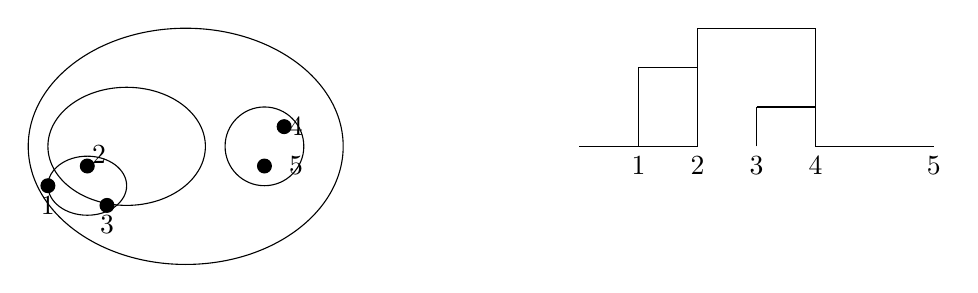
\begin{tikzpicture}[scale=0.5]
    \draw (0,0) ellipse (4 and 3);
    \draw (-1.5,0) ellipse (2 and 1.5);
    \draw (-2.5,-1) ellipse (1 and 0.75);
    \draw (2,0) ellipse (1 and 1);
    \filldraw [black] (-3.5,-1) circle (5pt);
    \filldraw [black] (-2.5,-0.5) circle (5pt);
    \filldraw [black] (-2,-1.5) circle (5pt);
    \filldraw [black] (2,-0.5) circle (5pt);
    \filldraw [black] (2.5,0.5) circle (5pt);
    \node at (-3.5,-1.5) {1};
    \node at (-2.2,-0.2) {2};
    \node at (-2,-2) {3};
    \node at (2.8,0.5) {4};
    \node at (2.8,-0.5) {5};
    \draw (10,0) -- (13,0) -- (13,3) -- (16,3) -- (16,0) -- (19,0);
    \draw (11.5,0) -- (11.5,2);
    \draw (14.5,0) -- (14.5,1);
    \draw (11.5,2) -- (13,2);
    \draw (14.5,1) -- (16,1);
    \node at (11.5,-0.5) {1};
    \node at (13,-0.5) {2};
    \node at (14.5,-0.5) {3};
    \node at (16,-0.5) {4};
    \node at (19,-0.5) {5};
\end{tikzpicture}

Hierarchical clustering is attractive for obvious reasons. To make matters even better, there are several simple agglomerative algorithms that can be used to construct them; we'll get to these shortly. But are the resulting clusterings any good? Or are they pretty arbitrary?

Let's make this more concrete. Pick any cost function for $k$-clustering, such as the $k$-center cost. Is it possible to construct a hierarchical clustering whose induced $k$-clustering is optimal for all $k$?

The answer is no. To see this, consider the following data set of six points. Below it are shown the optimal 2-clustering and the optimal 3-clustering. These are not nested within each other; therefore they are hierarchically incompatible.

This is bad news. Is it possible that imposing a hierarchical structure forces us to create bad intermediate clusterings? We'll now see that the situation isn't too bad, in that we can always construct a hierarchy that is close to optimal for all $k$.

\section*{4.2 Hierarchical clustering with the $k$-center cost function}

Recall the $k$-center cost function, set in a metric space $(\mathcal{X}, \rho)$.

\textbf{$k$-CENTER CLUSTERING}

\textbf{Input:} Finite set $S \subset \mathcal{X}$; integer $k$.

\textbf{Output:} $T \subset \mathcal{X}$ with $|T| = k$.

\textbf{Goal:} Minimize $\operatorname{cost}(T) = \max_{x \in S} \rho(x, T)$.

Let $\mathrm{OPT}_{k}$ denote the cost of the optimal $k$-center solution. We'll show how to construct a hierarchical clustering such that for all $k$, the induced $k$-clustering has cost $\leq 8 \mathrm{OPT}_{k}$.

\subsection*{4.2.1 Intuition}

We saw earlier that a 2-approximate solution to $k$-center can be obtained by farthest-first traversal. Let's use that traversal to number the points (start with any point, then pick the one farthest from it, then the one farthest from those two, and so on). Here's an example.

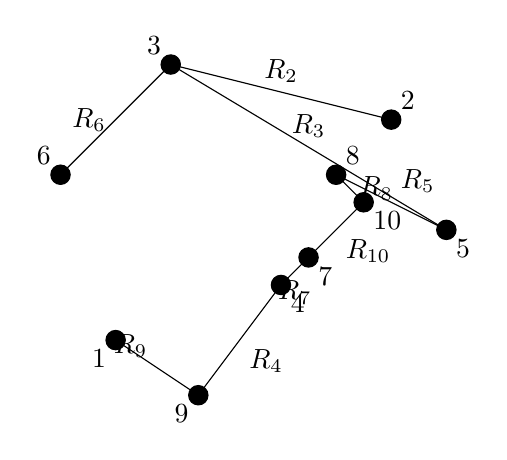
\begin{tikzpicture}[scale=0.7]
    \filldraw [black] (0,0) circle (5pt) node[below left] {1};
    \filldraw [black] (5,4) circle (5pt) node[above right] {2};
    \filldraw [black] (1,5) circle (5pt) node[above left] {3};
    \filldraw [black] (3,1) circle (5pt) node[below right] {4};
    \filldraw [black] (6,2) circle (5pt) node[below right] {5};
    \filldraw [black] (-1,3) circle (5pt) node[above left] {6};
    \filldraw [black] (3.5,1.5) circle (5pt) node[below right] {7};
    \filldraw [black] (4,3) circle (5pt) node[above right] {8};
    \filldraw [black] (1.5,-1) circle (5pt) node[below left] {9};
    \filldraw [black] (4.5,2.5) circle (5pt) node[below right] {10};
    \draw (0,0) -- node[above left] {$R_9$} (1.5,-1);
    \draw (1.5,-1) -- node[below right] {$R_4$} (3,1);
    \draw (3,1) -- node[below] {$R_7$} (3.5,1.5);
    \draw (3.5,1.5) -- node[below right] {$R_{10}$} (4.5,2.5);
    \draw (4.5,2.5) -- node[right] {$R_8$} (4,3);
    \draw (4,3) -- node[above right] {$R_5$} (6,2);
    \draw (6,2) -- node[above] {$R_3$} (1,5);
    \draw (1,5) -- node[left] {$R_6$} (-1,3);
    \draw (5,4) -- node[above] {$R_2$} (1,5);
\end{tikzpicture}

In this picture, $R_{i}$ is the distance from the $i$th point to its closest neighbor in $\{1, 2, \ldots, i-1\}$. So, $\operatorname{cost}(\{1, 2, \ldots, k\}) = R_{k+1}$, and we saw in an earlier lecture that $R_{k+1} \leq 2 \mathrm{OPT}_{k}$. Thus this farthest-first numbering gives us a 2-approximate $k$-clustering for all $k$. The hitch is that it is not hierarchical.

First let's figure out how to get a hierarchical clustering. In the picture, $i$ is connected to its closest neighbor $\pi(i) \in \{1, 2, \ldots, i-1\}$, thereby producing a tree structure. We can get a $k$-clustering by simply dropping the $k-1$ edges $2 \rightarrow \pi(2), 3 \rightarrow \pi(3), \ldots, k \rightarrow \pi(k)$, and treating each connected component as a cluster. These clusterings are indeed nested hierarchically. Let $T^{\pi}$ denote this hierarchical clustering.

The problem, however, is that the approximation ratio of these induced clusterings could be very bad. Instead, we set up the tree edges a bit differently. We connect each $i$ to a point $\pi'(i) \in \{1, 2 \ldots, i-1\}$ in such a way that the following property holds: any path with increasing node numbers has edge lengths of geometrically decreasing length.

We will build $\pi'$ by viewing the data at certain specific levels of granularity. Let $R = R_{2}$; this is some rough measure of the span of the data. If we do not care about distances smaller than $R$, the entire data set can be summarized by the single point $\{1\}$. This is our coarsest view, and we will call it $L_{0}$, granularity level zero. Suppose we want a little more detail, but we still don't care about distances less than $R / 2$. Then the data can be summarized by $L_{0}$ augmented with $L_{1} = \{i: R / 2 < R_{i} \leq R\}$. Continuing in this manner, we construct levels $L_{0}, L_{1}, L_{2}, \ldots$ such that every data point is within distance $R / 2^{j}$ of $L_{0} \cup L_{1} \cup \cdots \cup L_{j}$. Now define $\pi'(i)$ to be the closest point to $i$ at a lower level of granularity. We will show that $T^{\pi'}$ has provably good induced clusterings.

\subsection*{4.2.2 Algorithm}

\begin{verbatim}
Number the data points by farthest-first traversal
for i = 2, 3, ..., n:
    R_i = distance from i to its closest neighbor in {1, 2, ..., i-1}
R = R_2
for j > 1: L_j = {i: R / 2^j < R_i <= R / 2^{j-1}}
\pi'(i) = closest point to i at lower level of granularity
return T
\end{verbatim}

Figure 4.1 shows the effect of this algorithm on our earlier example.

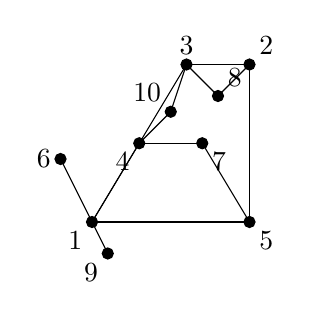
\begin{tikzpicture}[scale=0.4]
    \draw (0,0) -- (3,5);
    \draw (0,0) -- (5,0);
    \draw (5,0) -- (5,5);
    \draw (3,5) -- (5,5);
    \filldraw [black] (0,0) circle (5pt) node[below left] {1};
    \filldraw [black] (5,0) circle (5pt) node[below right] {5};
    \filldraw [black] (3,5) circle (5pt) node[above] {3};
    \filldraw [black] (5,5) circle (5pt) node[above right] {2};
    \filldraw [black] (1.5,2.5) circle (5pt) node[below left] {4};
    \filldraw [black] (2.5,3.5) circle (5pt) node[above left] {10};
    \filldraw [black] (3.5,2.5) circle (5pt) node[below right] {7};
    \filldraw [black] (4,4) circle (5pt) node[above right] {8};
    \filldraw [black] (0.5,-1) circle (5pt) node[below left] {9};
    \filldraw [black] (-1,2) circle (5pt) node[left] {6};
    \draw (0,0) -- (1.5,2.5);
    \draw (1.5,2.5) -- (2.5,3.5);
    \draw (2.5,3.5) -- (3,5);
    \draw (3,5) -- (4,4);
    \draw (4,4) -- (5,5);
    \draw (5,5) -- (5,0);
    \draw (5,0) -- (3.5,2.5);
    \draw (3.5,2.5) -- (1.5,2.5);
    \draw (0,0) -- (0.5,-1);
    \draw (0,0) -- (-1,2);
\end{tikzpicture}

\subsection*{4.2.3 Analysis}

\textbf{Lemma 1.} For any $i$, $\rho(i, \pi'(i)) \leq R / 2^{\operatorname{level}(i)-1}$.

\textbf{Proof.} Say $i \in L_{j}$. Let $l+1$ be the lowest-numbered point in $L_{j}$. Then $\rho(i, \pi'(i)) \leq R_{l+1} \leq R / 2^{j-1}$.

\textbf{Lemma 2.} For any $k$, the induced $k$-clustering has cost $\leq 4 R_{k+1} \leq 8 \mathrm{OPT}_{k}$.

\textbf{Proof.} Fix any $k$; the induced $k$-clustering has centers $1, 2, \ldots, k$.

Pick any $i$, and follow $\pi'$ pointers from $i$ up to some $q \in \{1, 2, \ldots, k\}$. Let $q'$ be the penultimate point on this path, right before $q$. Then

\begin{equation*}
\begin{aligned}
\rho(i, \{1, \ldots, k\}) &\leq \rho(i, q) \\
&\leq \rho(i, \pi'(i)) + \rho(\pi'(i), \pi'(\pi'(i))) + \cdots + \rho(q', q = \pi'(q')) \\
&\leq \frac{R}{2^{\operatorname{level}(i)-1}} + \frac{R}{2^{\operatorname{level}(\pi'(i))-1}} + \cdots + \frac{R}{2^{\operatorname{level}(q')-1}} \\
&\leq \frac{2R}{2^{\operatorname{level}(q')-1}} \leq 4 R_{k+1}.
\end{aligned}
\end{equation*}

For the last inequality: the level of $k+1$ is at most that of $q'$, so $R_{k+1} > R / 2^{\operatorname{level}(q')}$.

\textbf{Problem 1.} Find a better approximation algorithm for the hierarchical $k$-center problem.

\textbf{Problem 2.} Show lower bounds on the achievable approximation factor in hierarchical $k$-center. This might be a combination of a complexity-based lower bound (hardness of approximating $k$-center) and a structure-based lower bound (regardless of complexity, the hierarchical structure induces a certain amount of slack).

\section*{4.3 Agglomerative algorithms for hierarchical clustering}

The most popular algorithms for hierarchical clustering are agglomerative schemes:

\begin{itemize}
    \item Start with $n$ clusters, each a single data point.
    \item Repeat:
    \begin{itemize}
        \item Merge the two \"closest\" clusters.
    \end{itemize}
\end{itemize}

Crucial is the notion of distance between two clusters $C, C'$. Here are the most common choices:

\begin{enumerate}
    \item Single linkage: $\min \{\rho(i, j): i \in C, j \in C'\}$
    \item Complete linkage: $\max \{\rho(i, j): i \in C, j \in C'\}$
    \item Average linkage. This comes in three varieties. The last two require data in Euclidean space.
    \begin{enumerate}
        \item $\operatorname{mean} \{\rho(i, j): i \in C, j \in C'\}$
        \item $\|\operatorname{mean}(C) - \operatorname{mean}(C')\|^{2}$
        \item (Ward's method) $\frac{|C| \cdot |C'|}{|C| + |C'|} \|\operatorname{mean}(C) - \operatorname{mean}(C')\|^{2}$
    \end{enumerate}
\end{enumerate}

\subsection*{4.3.1 Single linkage}

Imagine a process in which a \"distance knob\" is slowly turned up from zero to infinity. Initially, the $n$ data points are not connected. When the knob passes $r$, edges are placed between points at distance $r$ from each other. The clustering at any point in time is specified by the connected components of the graph at that time. These are exactly the clusterings induced by single linkage.

This is equivalent to running Kruskal's algorithm on the data points, using interpoint distances as edge weights. To get a $k$-clustering, drop the $k-1$ largest edges in the minimum spanning tree and output the resulting connected components.

Single linkage has a variety of attractive properties in theory, some of which we will see quite shortly. But in practice it has a disastrous tendency to form long chains.

\subsection*{4.3.2 Complete linkage}

Complete linkage can be thought of as a greedy agglomerative heuristic for hierarchical $k$-center: it always does the merge that results in the smallest maximum diameter. It is known that its induced $k$-clusterings are not necessarily close to the optimal $k$-clusterings in terms of $k$-center cost: there are examples in which the gap is a multiplicative factor of $k / 2$ (for $k \approx \log n$). However, this gap can be shown to be at most $k^{\log_{2} 3}$.

\textbf{Problem 3.} Obtain matching upper and lower bounds for the approximation factor of complete linkage.

\subsection*{4.3.3 Ward's method of average linkage}

Ward's method always does the merge that leads to the smallest increase in $k$-means cost. To see this, start by fixing any data set $S \subset \mathbb{R}^{d}$, and recall the $k$-means cost function: for $T \subset \mathbb{R}^{d}$,

\begin{equation*}
\operatorname{cost}(T) = \sum_{x \in S} \min_{t \in T} \|x - t\|^{2}.
\end{equation*}

\textbf{Lemma 3.} For any sets $C, C' \subset \mathbb{R}^{d}$,

\begin{equation*}
\operatorname{cost}(C \cup C') = \operatorname{cost}(C) + \operatorname{cost}(C') + \frac{|C| \cdot |C'|}{|C| + |C'|} \|\operatorname{mean}(C) - \operatorname{mean}(C')\|^{2}.
\end{equation*}

\textbf{Proof.} Let $\mu = \operatorname{mean}(C)$, $\mu' = \operatorname{mean}(C')$, and $\bar{\mu} = \operatorname{mean}(C \cup C')$.

\begin{equation*}
\begin{aligned}
&\operatorname{cost}(C \cup C') - \operatorname{cost}(C) - \operatorname{cost}(C') \\
&= \sum_{x \in C \cup C'} \|x - \bar{\mu}\|^{2} - \sum_{x \in C} \|x - \mu\|^{2} - \sum_{x \in C'} \|x - \mu'\|^{2} \\
&= \sum_{x \in C} (\|x - \bar{\mu}\|^{2} - \|x - \mu\|^{2}) + \sum_{x \in C'} (\|x - \bar{\mu}\|^{2} - \|x - \mu'\|^{2}) \\
&= |C| \cdot \|\mu - \bar{\mu}\|^{2} + |C'| \cdot \|\mu' - \bar{\mu}\|^{2} \\
&= |C| \cdot \left\|\frac{|C'|}{|C| + |C'|} (\mu' - \mu)\right\|^{2} + |C'| \cdot \left\|\frac{|C|}{|C| + |C'|} (\mu - \mu')\right\|^{2} \\
&= \frac{|C| \cdot |C'|}{|C| + |C'|} \|\mu - \mu'\|^{2}.
\end{aligned}
\end{equation*}

The third equality uses a special property of squared Euclidean distances that we saw in the lecture on $k$-means. The fourth equality uses $\bar{\mu} = (|C| \mu + |C'| \mu') / (|C| + |C'|)$.

\textbf{Problem 4.} How good an approximation to the optimal $k$-means clustering is the induced $k$-clustering of Ward's method?

\textbf{Problem 5.} All these agglomerative hierarchical schemes seem to require $O(n^{2})$ time, which is prohibitive for massive data sets. Find good ways to speed them up, based on (a) data structures for fast nearest neighbor search, or (b) clever sampling methods.

\end{document}
